\documentclass[final]{article}

% if you need to pass options to natbib, use, e.g.:
% \PassOptionsToPackage{numbers, compress}{natbib}
% before loading nips_2017
%
% to avoid loading the natbib package, add option nonatbib:
% \usepackage[nonatbib]{nips_2017}

\usepackage{nips_2017}

% to compile a camera-ready version, add the [final] option, e.g.:
% \usepackage[final]{nips_2017}

\usepackage[utf8]{inputenc} % allow utf-8 input
\usepackage[T1]{fontenc}    % use 8-bit T1 fonts
\usepackage{hyperref}       % hyperlinks
\usepackage{url}            % simple URL typesetting
\usepackage{booktabs}       % professional-quality tables
\usepackage{amsfonts}       % blackboard math symbols
\usepackage{nicefrac}       % compact symbols for 1/2, etc.
\usepackage{microtype}      % microtypography

% \usepackage{lmodern}

\usepackage{tikz}
\usepackage{float}
\usetikzlibrary{shapes, arrows}

\title{Formatting instructions for NIPS 2017}

% The \author macro works with any number of authors. There are two
% commands used to separate the names and addresses of multiple
% authors: \And and \AND.
%
% Using \And between authors leaves it to LaTeX to determine where to
% break the lines. Using \AND forces a line break at that point. So,
% if LaTeX puts 3 of 4 authors names on the first line, and the last
% on the second line, try using \AND instead of \And before the third
% author name.

\author{
  Forest Kobayashi \\
  Department of Mathematics\\
  Harvey Mudd College\\
  Claremont, CA 91711 \\
  \texttt{fkobayash@hmc.edu} \\
  %% examples of more authors
  \And
  Jacky Lee \\
  Department of Mathematics\\
  Department of Computer Science \\
  Harvey Mudd College \\
  Claremont, CA 91711 \\
  \texttt{jaclee@hmc.edu}
}

\begin{document}
% \nipsfinalcopy is no longer used

\maketitle

\begin{abstract}
  Stock data is very difficult to analyze using classical methods, in
  large part due to heavy involvement of humans in stock pricing. In
  this paper, we examine a new approach to analyzing time-series stock
  data, particularly in the context of grouping correlated stocks.
\end{abstract}

\section{Introduction}
Here is a rough table of contents for our paper, so that the reader
has a rough idea of where we'll be going:
\begin{enumerate}
\item Motivation (challenges to modelling stock data)
\item Long-term goal for the model / ideal model architecture
\item Classification
\item Findings
\item Conclusion
\end{enumerate}

\section{}

\section{Goal for the Model}
Our large-scale goal for the model is as follows:
\begin{figure}[H]
  \centering
    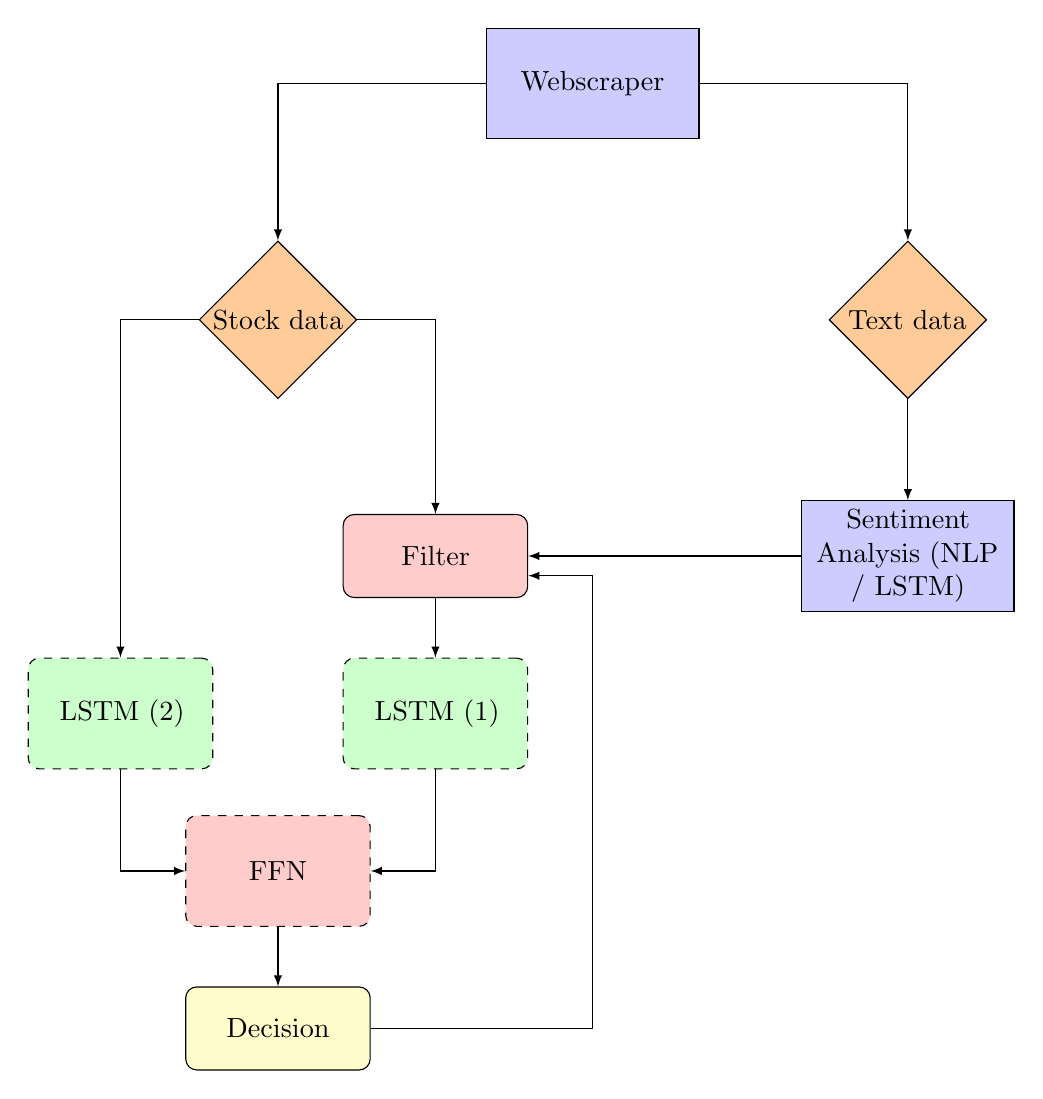
\begin{tikzpicture}[node distance = 2cm, auto]
      \tikzstyle{data} = [
        diamond,
        draw,
        fill=orange!40,
        text width = 5em,
        text badly centered,
        node distance = 3cm,
        inner sep = 0pt
      ]

      \tikzstyle{code} = [
        rectangle,
        draw,
        fill=blue!20,
        text width=7em,
        text centered,
        minimum height=4em
      ]

      \tikzstyle{network} = [
        rectangle,
        draw,
        dashed,
        fill=green!20,
        text width = 6em,
        text centered,
        rounded corners,
        minimum height = 4em
      ]

      \tikzstyle{feedforward} = [
        rectangle,
        draw,
        dashed,
        fill=red!20,
        text width = 6em,
        text centered,
        rounded corners,
        minimum height = 4em
      ]

      \tikzstyle{filter} = [
        draw,
        rectangle,
        fill=red!20,
        text width = 6em,
        text centered,
        minimum height=3em,
        rounded corners
      ]

      \tikzstyle{decision} = [
        draw,
        rectangle,
        fill=yellow!20,
        text width = 6em,
        text centered,
        minimum height=3em,
        rounded corners
      ]

      \node[code] (webscraper) at (0,6) {Webscraper};
      \node[data] (time series) at (-4,3) {Stock data};
      \node[data] (text) at (4,3) {Text data};
      \node[code] (processer) at (4,0) {Sentiment Analysis (NLP /
        LSTM)};
      \node[filter] (filter) at (-2,0) {Filter};
      \node[network] (lstm1) at (-2,-2) {LSTM (1)};
      \node[network] (lstm2) at (-6,-2) {LSTM (2)};
      \node[feedforward] (feedforward) at (-4,-4) {FFN};

      \node[decision] (decision) at (-4,-6) {Decision};

      \draw[-latex] (webscraper) -| (time series);
      \draw[-latex] (webscraper) -| (text);
      \draw[-latex] (text) -- (processer);
      \draw[-latex] (time series) -| (filter);
      \draw[-latex] (filter) -- (lstm1);
      \draw[-latex] (processer) -- (filter);
      \draw[-latex] (time series) -| (lstm2);
      \draw[-latex] (lstm2) |- (feedforward);
      \draw[-latex] (lstm1) |- (feedforward);
      \draw[-latex] (feedforward) -- (decision);
      \draw (decision) -- (0,-6) -- (0,-.25);
      \draw[-latex] (0,-.25) -- (-.82,-.25);
    \end{tikzpicture}
  \caption{Goal for the model}
  \label{fig:goal}
\end{figure}

\section{Classification}
Using LSTMs to predict stock pricing is, for the most part, a solved
problem. Implementations and hyperparameters may differ, of course,
but underneath, the structure of the model is largely the same. Hence,
we decided to focus our work on augmenting the LSTM
\subsection{Frequency Analysis}


\end{document}
